\begin{singlespacing}
\chapter{A search for new phenomena}
\label{chapter:2ljets}
%
\begin{epigraphs}
\qitem{%
An experiment is never a failure solely because it fails to
achieve predicted results. An experiment is a failure only when it also
fails adequately to test the hypothesis in question, when the data it
produces don’t prove anything one way or another.%
}%
{Robert M. Pirsig~\cite{pirsig1999zen}}
\qitem{%
But there is one feature I notice that is generally missing in cargo cult
science. \ldots\
% That is the idea that we all hope you have learned in studying science in
% school--we never say explicitly what this is, but just hope that you catch
% on by all the examples of scientific investigation. It is interesting,
% therefore, to bring it out now and speak of it explicitly.
It's a kind of scientific integrity, a principle of scientific thought that
corresponds to a kind of utter honesty --- a kind of leaning over backwards.%
}%
{Richard Feynman~\cite{feynman1974cargo}}
\end{epigraphs}
\end{singlespacing}


% begin with physics content and results

Our main result is the content of Figure~\ref{fig:2ljets_summary}, which shows
the data in all main regions of this analysis, along with the regions' names,
and post-fit background expectations.
This figure illustrates the background-only part of a \clown{likelihood}
model which is extended with signals to test alternative models.

We use two signal models in the $\twoljets$ electroweak analysis.
One is an MSSM chargino-neutralino model (C1N2) which acts to produce
$\chargino{1}\textrm{--}\neutralino{2}$ pairs which decay via $W$ and $Z$
channels respectively to jets and a lepton pair.
The other is a GMSB model which decays via Higgs and $Z$ bosons in variable
branching fractions.
Diagrams illustrating the C1N2 and GMSB signal models we consider are shown in
Figure~\ref{fig:2ljets_signal_diagrams}.
Some example effects of these signals in signal regions are displayed in
Figure~\ref{fig:2ljets_signal_examples}.


At each parameter point of a signal model, it is added to the background model
and tested against data in the $\mathrm{CLs}$ prescription.
Contours showing which regions where those tests label the signal model
parameters as excluded excluded are shown for
C1N2 in Figure~\ref{fig:2ljets_contours_c1n2} and for
GMSB in~\ref{fig:2ljets_contours_gmsb}.

Data in discovery regions are presented and interpreted in
Table~\ref{tab:2ljets_discovery}.


% summary plot

\begin{figure}[tp]
\centering
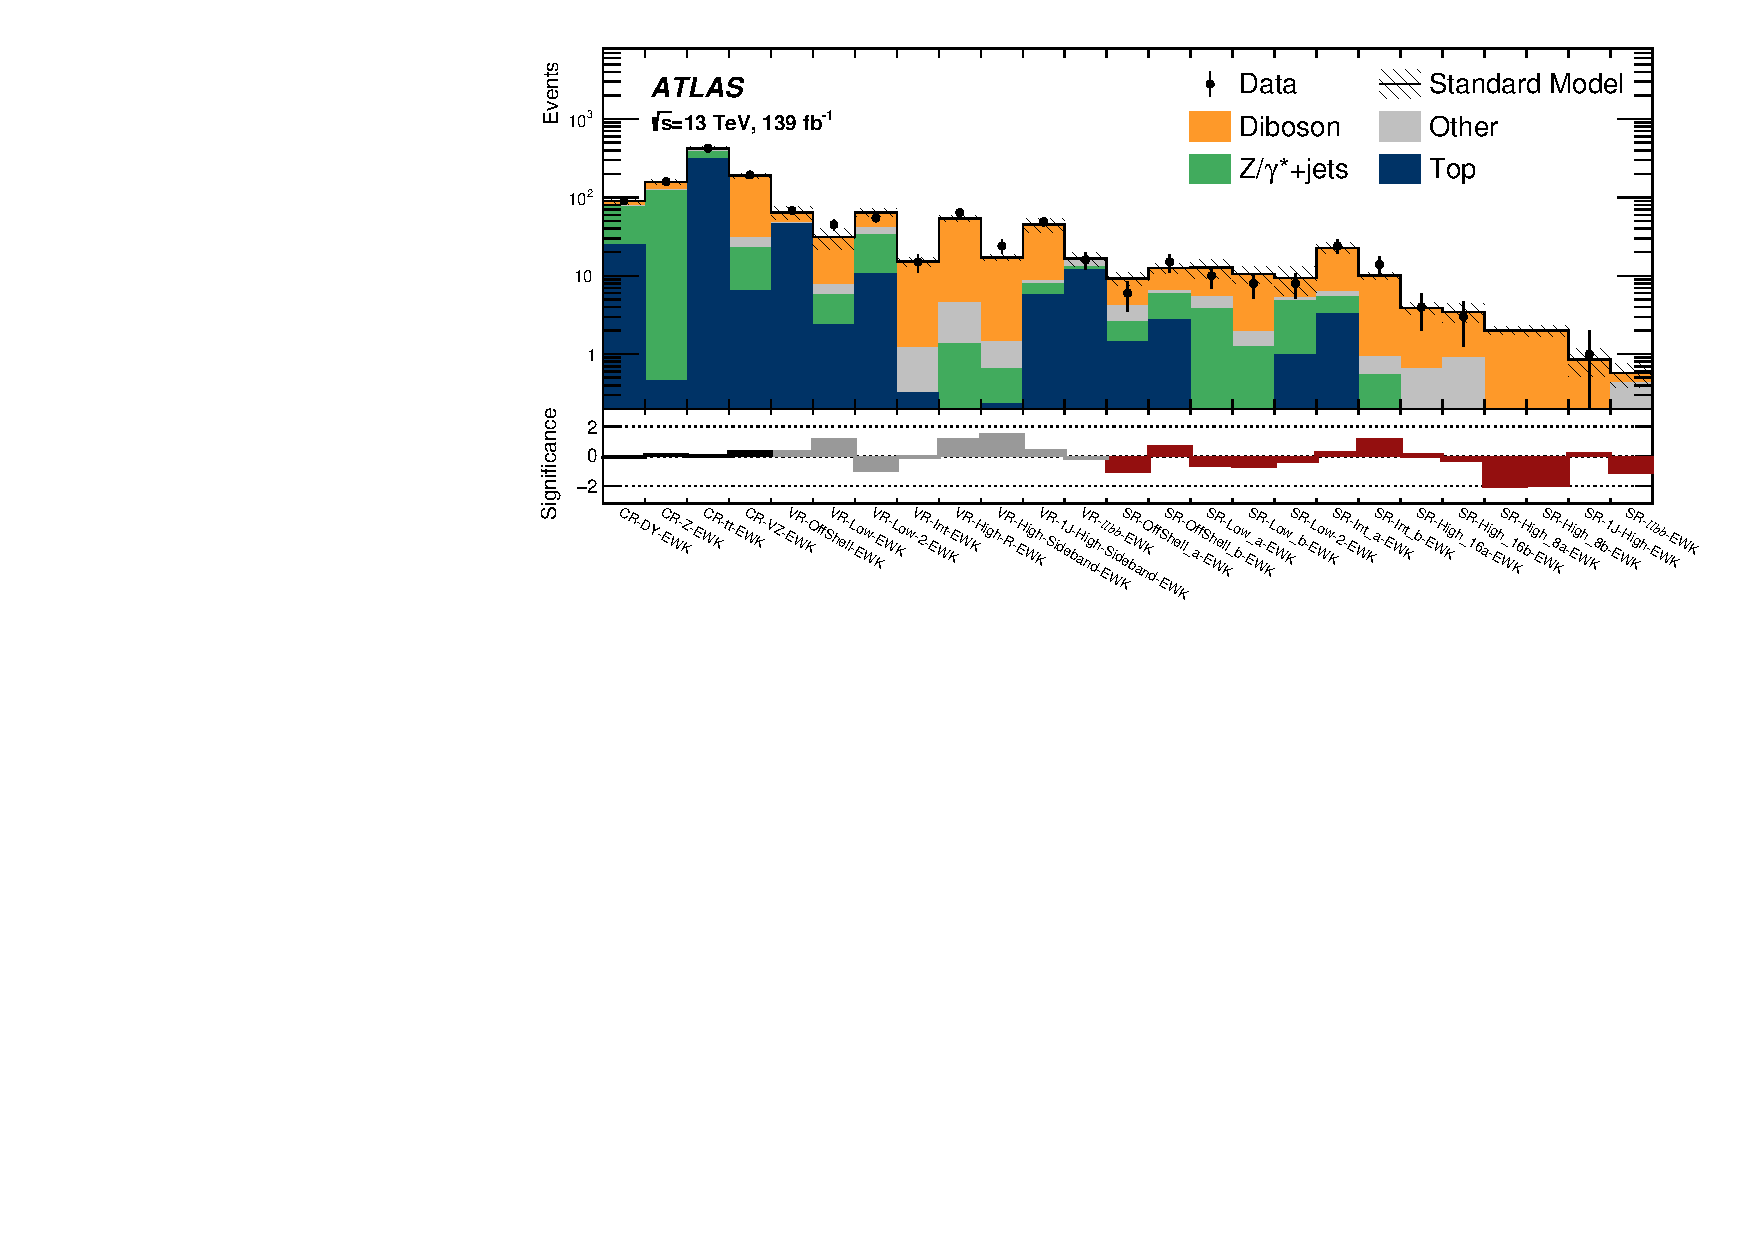
\includegraphics[width=\textwidth]{figures/2ljets_summary_log.pdf}
\caption{%
Data of the $\twoljets$ electroweak analysis with \emph{post-fit} backgrounds
for which the lower panel shows $S_\mathrm{ATLAS}$ from
Equation~\ref{eqn:significance_atlas}.
Control, validation and signal regions are shown from left to right, with the
regions within each category ordered approximately by their typical $\etmiss$.
Likelihoods from validation regions are not included in the fit.
The `Top' category contains $t\bar t$ and $tW$ processes, and
`Other' contains fake/non-prompt lepton, higgs, triboson, $t\bar tZ$, and other
rare top processes.%
}
\label{fig:2ljets_summary}
\end{figure}


% signal diagrams

\begin{figure}[t]
\centering
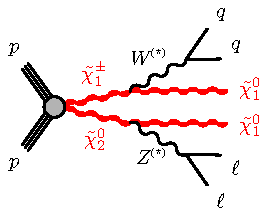
\includegraphics[width=0.48\textwidth]{figures/2ljets_c1n2_llqqn1n1_wz.pdf}
\hfill
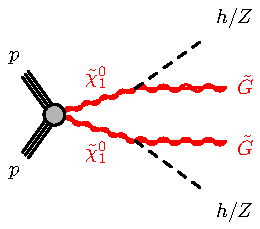
\includegraphics[width=0.45\textwidth]{figures/2ljets_n1n1_hhggzz.pdf}
\caption{%
Supersymmetric signal processes in the $\twoljets$ electroweak analysis.
\\[0.5em]
Left: C1N2, where the initial $\chargino{1}\textrm{--}\neutralino{2}$ pair
is produced through a $s$-channel $W^{\pm}$ resonance and the masses of
weak bosons in decays are bounded by the mass splitting
$m(\chargino{1}, \neutralino{2}) - m(\neutralino{1})$.
We explore the parameters
$m(\chargino{1}, \neutralino{2})$ and $m(\neutralino{1})$.
\\[0.5em]
Right: GMSB, where the initial $\neutralino{1}\textrm{--}\neutralino{1}$ pair
is produced by soft decays from pairs including $\chargino{1}$,
$\neutralino{2}$ or $\neutralino{1}$.
Although the $h$ and $Z$ bosons decay to many states, we target
$Z\rightarrow \ell\ell$ with
$h/Z\rightarrow bb/jj$.
We explore the parameters
$m(\neutralino{1})$ and $B(\neutralino{1} \rightarrow h \tilde{G})$ with fixed
$m(\chargino{1}, \neutralino{2}) - m(\neutralino{1}) = 1~\eV[G]$.
}
\label{fig:2ljets_signal_diagrams}
\end{figure}


% signal region plots

\begin{figure}[tp]
\centering
\begin{subfigure}{0.49\textwidth}
    \centering
    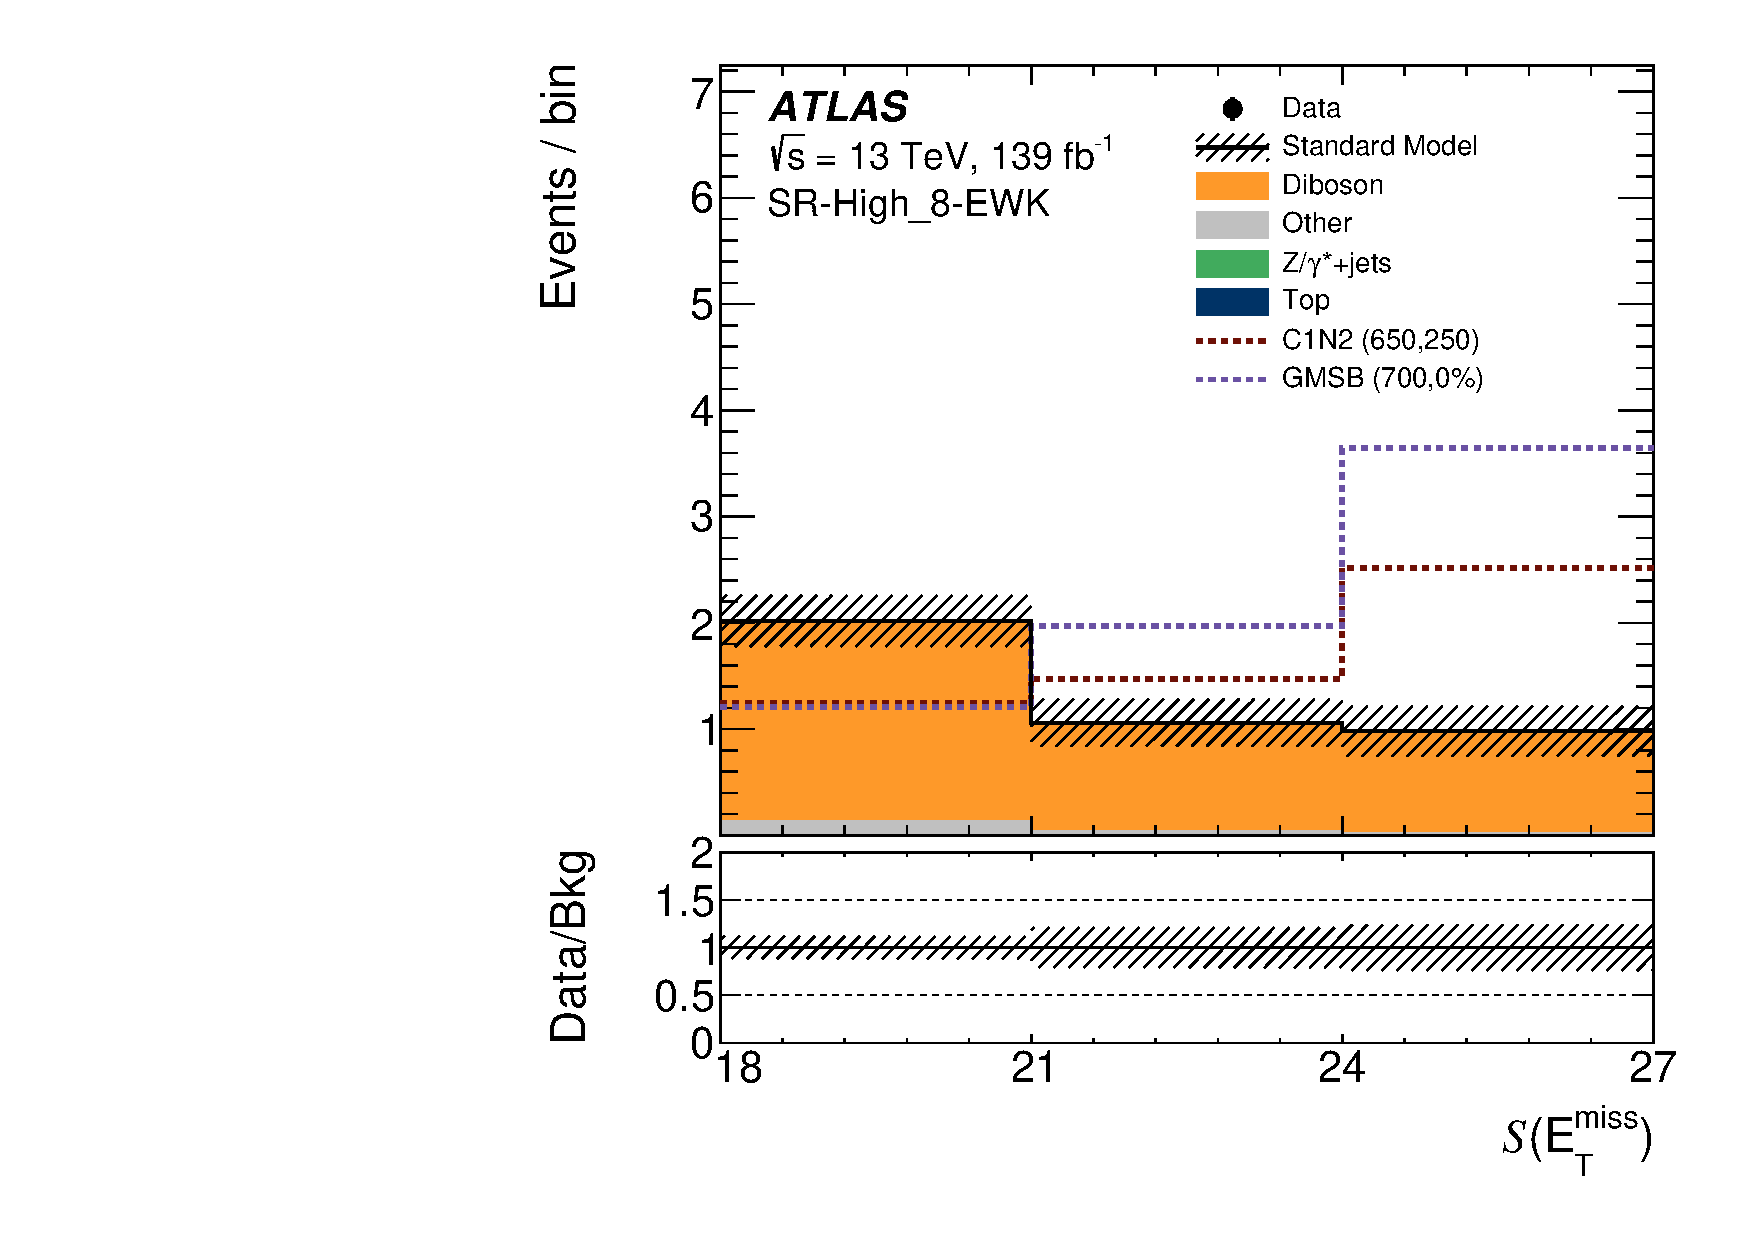
\includegraphics[width=\textwidth]{figures/2ljets_sr_high_8_met_sig.pdf}
    \caption{SR-High-8}
\end{subfigure}
\hfill
\begin{subfigure}{0.49\textwidth}
    \centering
    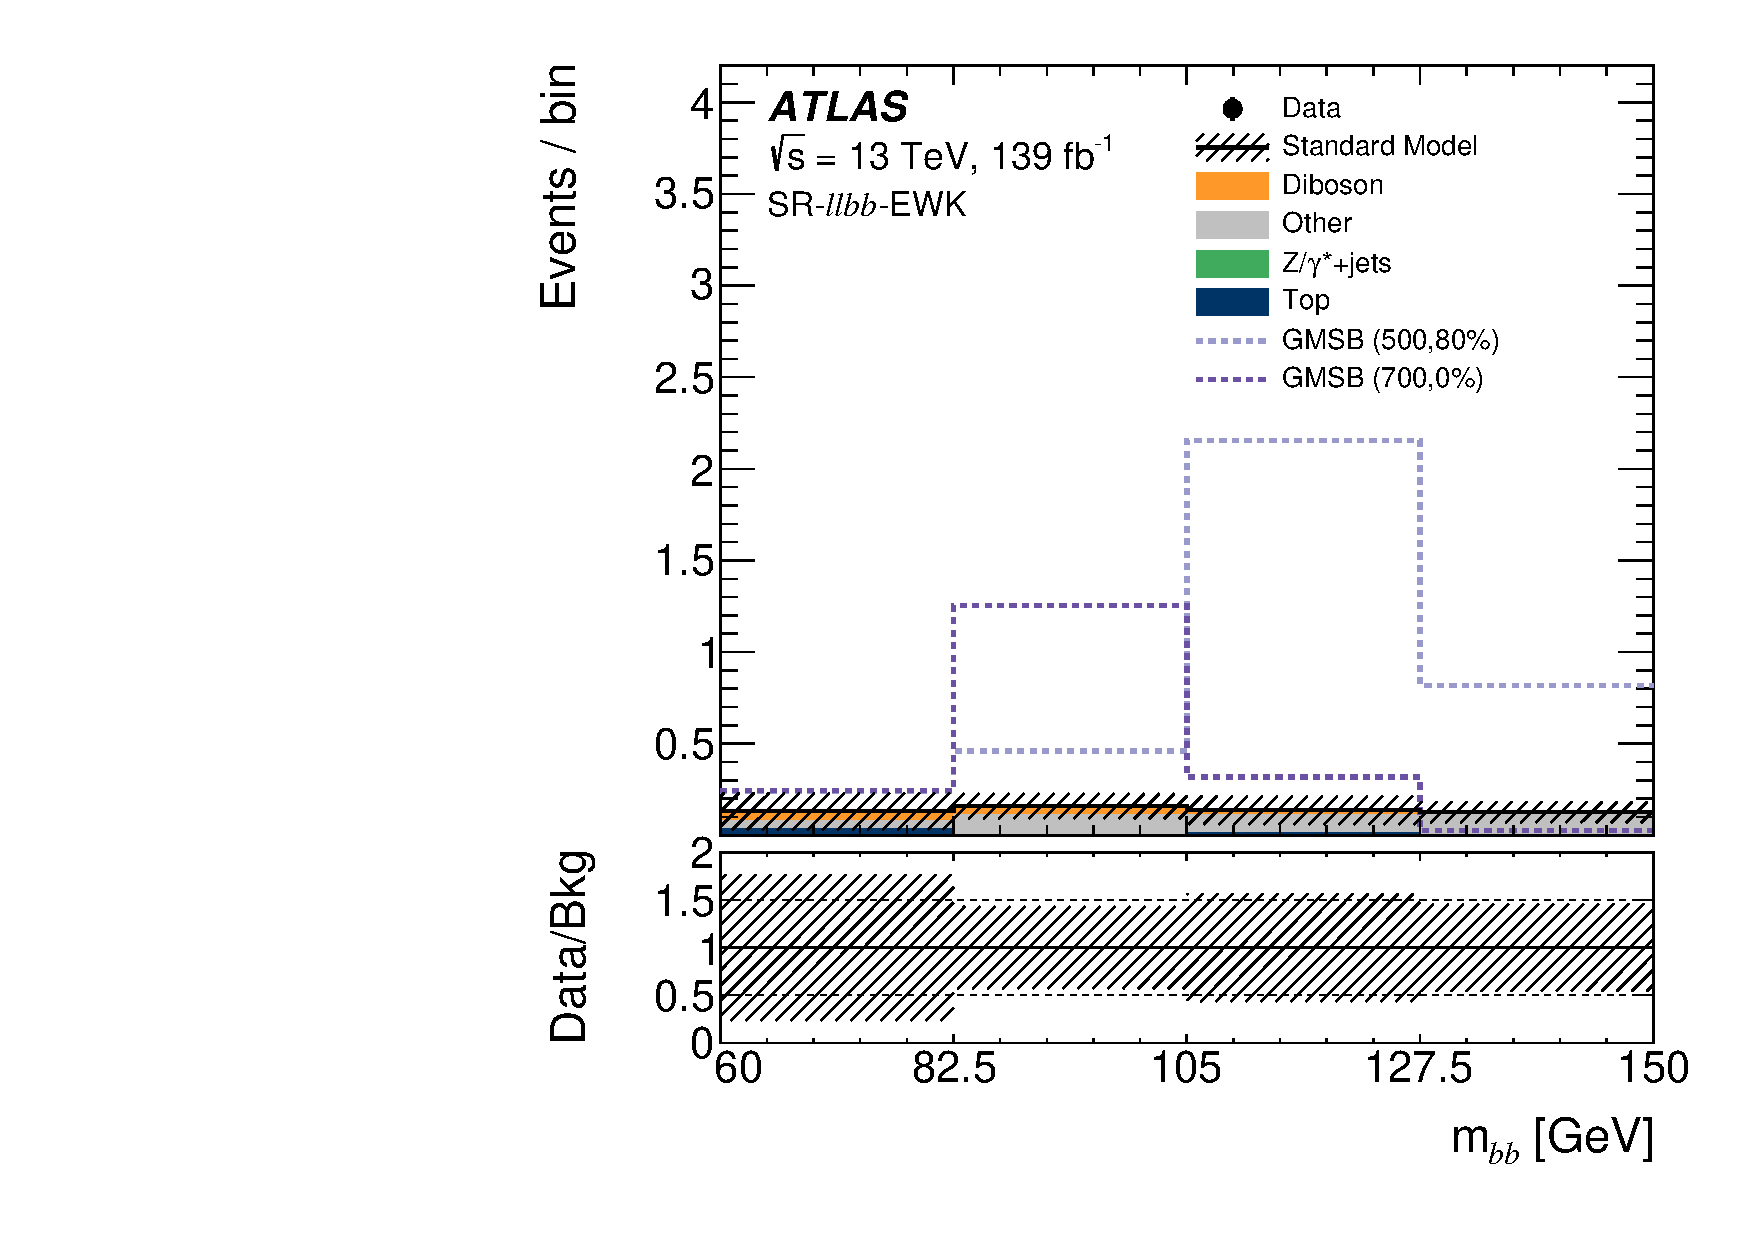
\includegraphics[width=\textwidth]{figures/2ljets_sr_llbb_mbb.pdf}
    \caption{SR-$\ell\ell bb$}
\end{subfigure}
\\[0.5em]
\begin{subfigure}{0.49\textwidth}
    \centering
    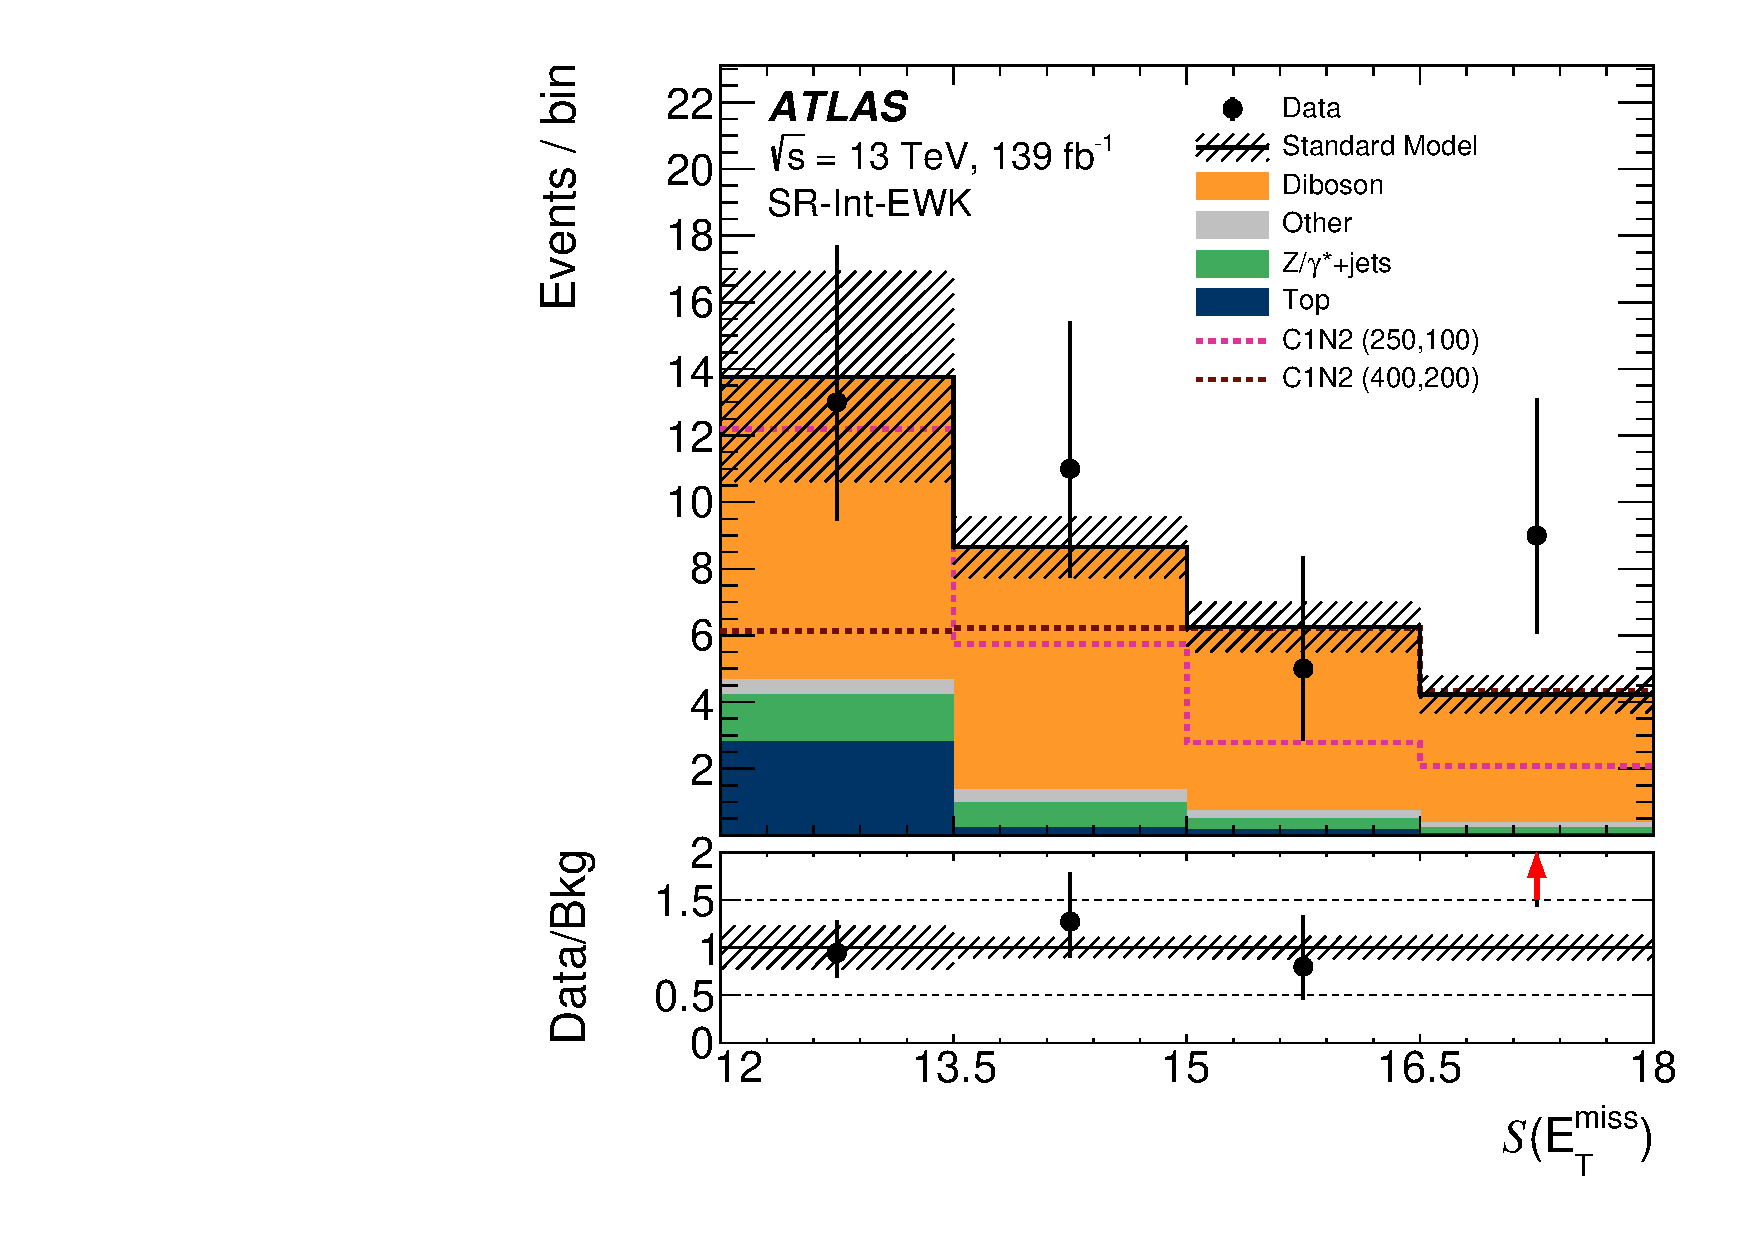
\includegraphics[width=\textwidth]{figures/2ljets_sr_int_met_sig.pdf}
    \caption{SR-Int}
\end{subfigure}
\hfill
\begin{subfigure}{0.49\textwidth}
    \centering
    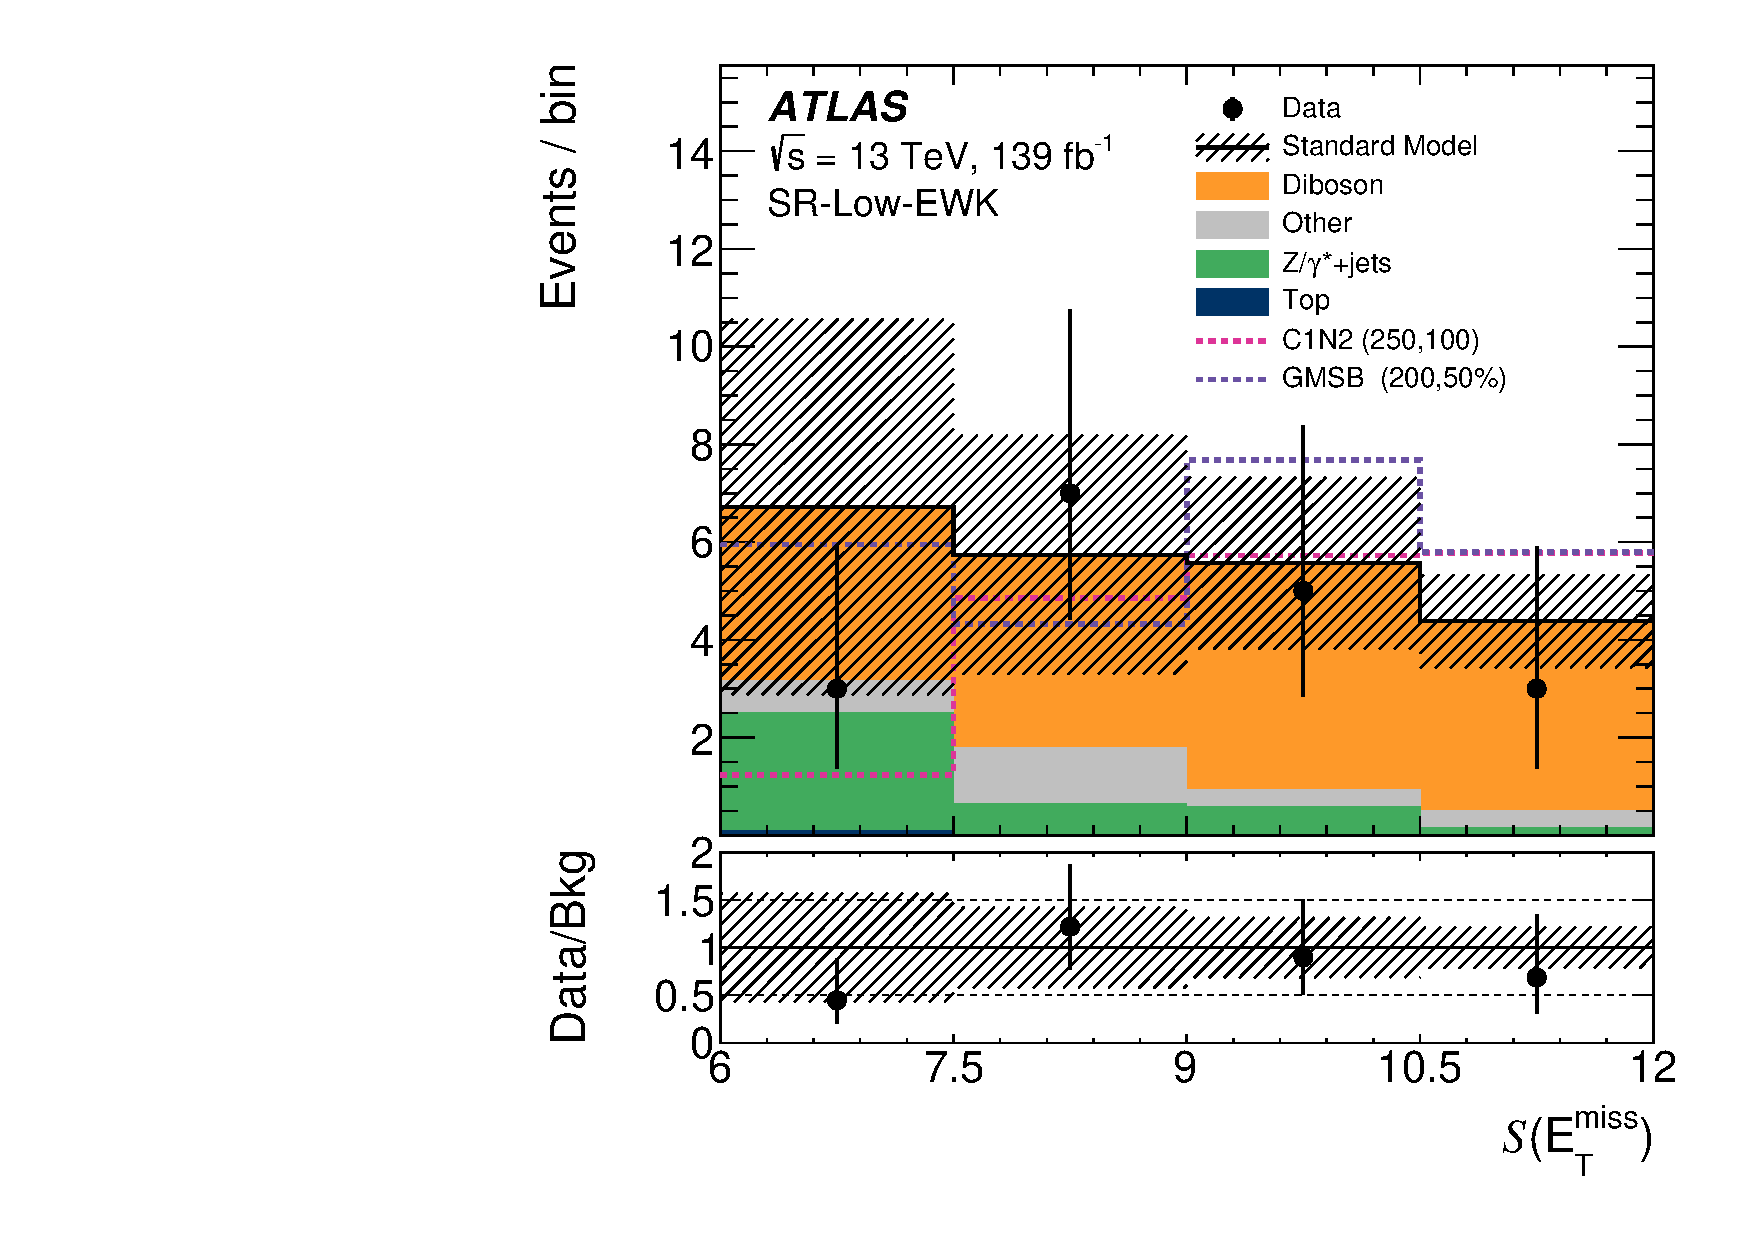
\includegraphics[width=\textwidth]{figures/2ljets_sr_low_met_sig.pdf}
    \caption{SR-Low}
\end{subfigure}
\caption{%
Example signal region histograms with benchmark signal sample yields overlaid
as dotted lines.
Physically, signal yields would add on top of the backgrounds.
Data are shown; regions in the the top two plots observe zero data, and the
Poisson error bars for $0$ events are hidden for aesthetic reasons.
}
\label{fig:2ljets_signal_examples}
\end{figure}



% exclusion plots

\begin{figure}[tp]
\centering
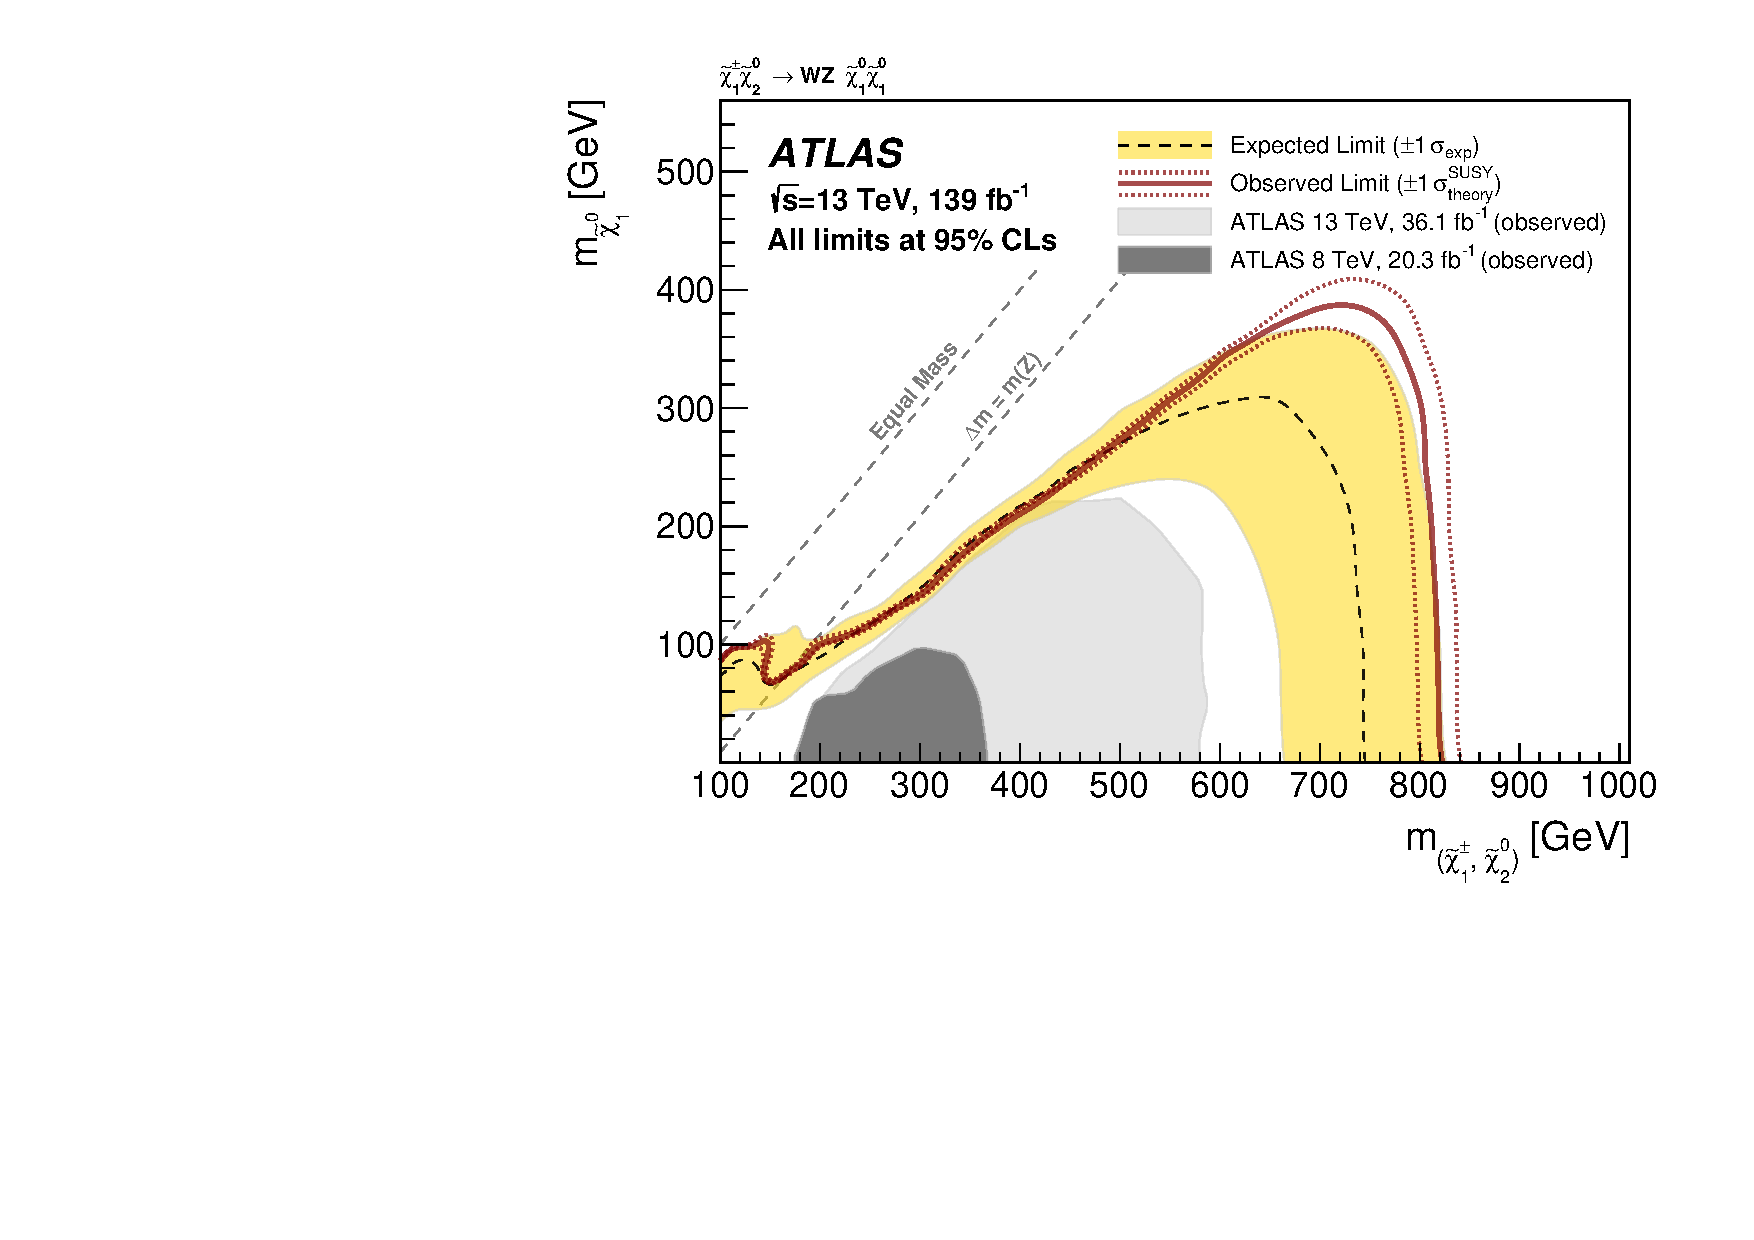
\includegraphics[width=0.99\textwidth]{figures/2ljets_contours_c1n2.pdf}
\caption{%
Contours for the C1N2 model in the $\twoljets$ electroweak analysis.
Space below the solid red line is labelled as excluded and its dotted
neighbours show the result if all signal cross-sections are varied up and down
by theoretical error bars.
The yellow band shows the $\pm1$-sigma region of exclusion contours
from asymptotic approximations to the prior distribution of the test statistic.
Grey areas are observed limits from the two-lepton parts
of~\cite{SUSY-2016-24} and~\cite{SUSY-2013-11}.
Exclusion is defined by the $95\%$ $\mathrm{CLs}$ prescription
in asymptotic approximations.
All contours are interpolated from a sparse grid.
}
\label{fig:2ljets_contours_c1n2}
\end{figure}

\begin{figure}[tp]
\centering
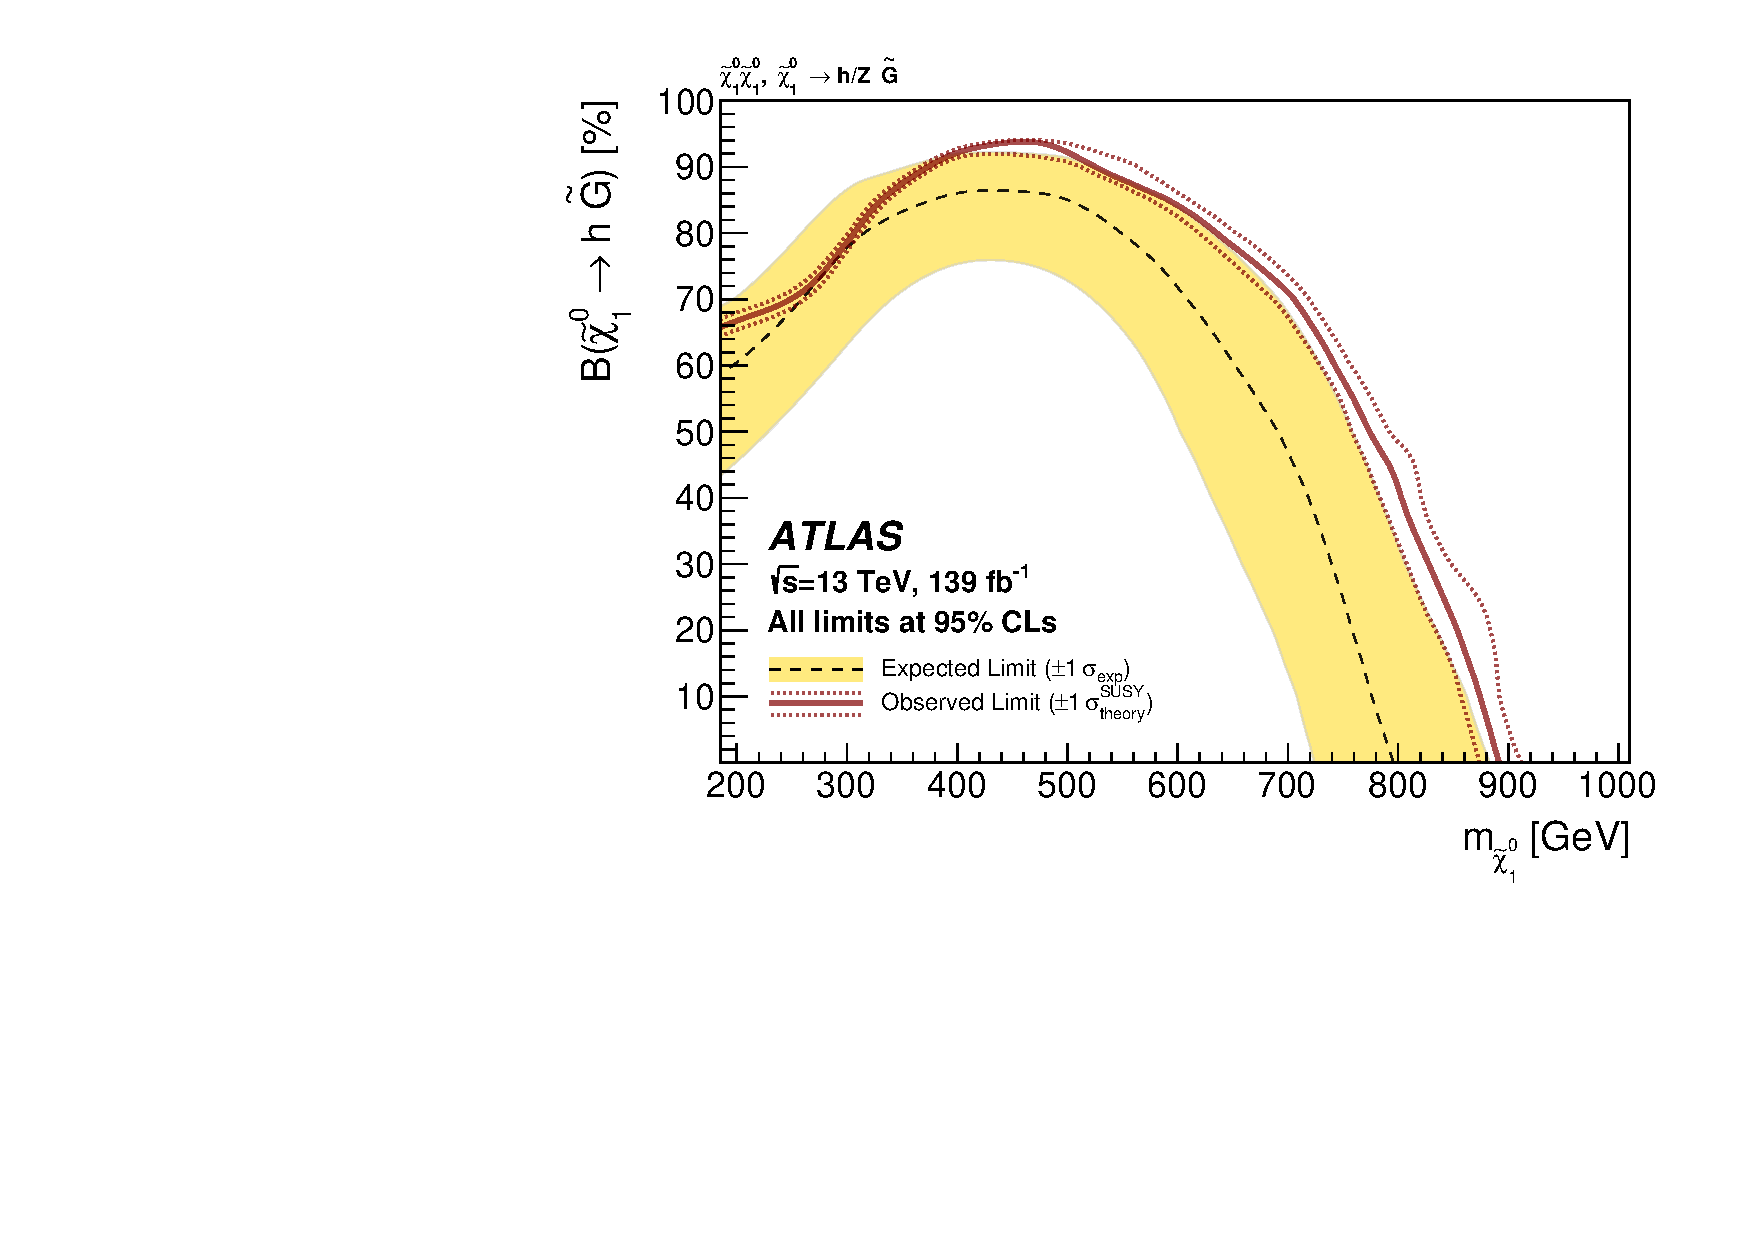
\includegraphics[width=0.99\textwidth]{figures/2ljets_contours_gmsb.pdf}
\caption{%
Contours for the GMSB model in the $\twoljets$ electroweak analysis.
Space below the solid red line is labelled as excluded and its dotted
neighbours show the result if all signal cross-sections are varied up and down
by theoretical error bars.
The yellow band shows the $\pm1$-sigma region of exclusion contours
from asymptotic approximations to the prior distribution of the test statistic.
Exclusion is defined by the $95\%$ $\mathrm{CLs}$ prescription
in asymptotic approximations.
All contours are interpolated from a sparse grid.
}
\label{fig:2ljets_contours_gmsb}
\end{figure}


% upper limits
% definitely want this after pictures
\FloatBarrier
\begin{table}[tp]
\centering
% custom separator for aligned +-
% https://stackoverflow.com/a/2132998
\begin{tabular*}{\textwidth}{lr@{$~\pm~$}lcccccc}
Region &
\multicolumn{2}{c}{Fitted} &
Data &
$\langle A\epsilon{ \sigma}\rangle_{\mathrm{obs}}^{95}~\mathrm{fb}$ &
$S_{\mathrm{obs}}^{95}$  &
$S_{\mathrm{exp}}^{95}$ &
$\mathrm{CLb}$ &
$p(s=0)$  \\[1.5ex]
DR-OffShell      & $22.1$ & $2.7$ & 21 & $0.10$ & $14.3$ & $12.3^{+4.7}_{-3.1}$ & $0.68$ & $0.50$ \\[.5ex]
DR-Low           & $22$ & $4$ & 18 & $0.08$ & $10.8$ & $15.3^{+5.7}_{-4.0}$ & $0.09$ & $0.50$ \\[.5ex]
DR-Int           & $35$ & $4$ & 38 & $0.15$ & $20.9$ & $17.5^{+5.9}_{-3.9}$ & $0.73$ & $0.23$ \\[.5ex]
DR-High          & $3.9$ & $0.5$  & 0  & $0.02$ & $3.0$ & $5.6^{+2.2}_{-1.5}$ & $0.00$ & $0.50$ \\[.5ex]
DR-$\ell\ell bb$ & $0.51$ & $0.20$  & 0  & $0.02$ & $3.0$ & $3.0^{+1.3}_{-0.0}$ & $0.19$ & $0.50$ \\[.5ex]
\end{tabular*}
\caption{%
Upper limit results in discovery region.
The fitted yield is in the background-only model constrained by the data in each region.
Limits are intended to reflect constrains on additive signal contributions.
\\[0.5em]
Left to right:
the region name,
the post-fit background expectation,
the number of data observed,
the observed $95\%$ $\mathrm{CLs}$ upper limit on the visible cross-section
$\langle\epsilon\sigma\rangle_\mathrm{obs}^{95}$,
its corresponding signal expectation $S_\mathrm{obs}^{95}$,
the \clown{expected} $95\%$ upper limits on the signal expectation $S_\mathrm{exp}^{95}$
as would be obtained were the test statistic given by its central or
$\pm1$-sigma variations,
$\mathrm{CLb}$ evaluated with the signal expectation set to the observed upper limit,
and the discovery $p$-value (capped at $0.5$) with its equivalent significance.
\\[0.5em]
Upper limits use the one-sided profile likelihood test statistic.
The discovery $p$-value uses a profile likelihood test statistic in a one-sided test.
All $p$-values are estimated by simulation of alternative data.
\TODO{add labels and references to asymptotic formulae paper}
}
\label{tab:2ljets_discovery}
\end{table}


\paragraph{My contributions}
\begin{itemize}
\item Design, implementation and execution of the electroweak part of the analysis.
\item Analysis Contact from January to October 2020.
\item Production of main data inputs for all three analyses
and the RJR $3\ell$ search \TODO{cite}.
I produced all systematic variations for the background samples and all
electroweak signal samples.
Other group members assisted with the central background sample.
\item Integration with ATLAS combinations and pMSSM scan efforts by
performing their validation studies and serializing the analysis results.
\item Preparation of electroweak results for publication in the paper, and the
public HEPData record~\cite{maguire2017hepdata}.
\end{itemize}

\clearpage
\FloatBarrier
\section{Context}
% previous results on 2(/3)L from ATLAS
% other constraints on these models from ATLAS/CMS
% previous region design, motivation for this work


\section{Event variables}
% lepton, jet definitions



Uncomfortably many event variables are used to define the regions of this
analysis.
Definitions of these variables are collected here.
All variables with a double object subscript (such as $\mll$, $\rjj$) refer to
the first two of those particles when ordered in decreasing $\pt$.
\begin{itemize}
\item $\etmiss$: missing transverse momentum.
\item $\etmisssig$: object-based missing transverse momentum significance.
It scales $\etmiss$ by an uncertainty derived from the resolutions of
reconstructed objects~\cite{atlas_met_significance}.
\item $\mll$: invariant mass of the hardest two leptons.
\item $\mjj$: invariant mass of the two hardest jets.
\item $\mbb$: invariant mass of the two hardest b-tagged jets.
\item $\mjetone$: mass of the hardest jet.
% TODO
% \item $\Rll$: estimated angular distance in $\eta,\phi$ between the lepton pair.
% \item $\Rjj$: estimated angular distance in $\eta,\phi$ between the two hardest jets.
% \item $\Delta\phi(p_{\ell\ell}, \Etmiss)$: estimated distance in azimuthal
% angle between the vector sum of the lepton pair and the missing transverse momentum.
% \item $\mttwo(\ell, \ell; 0)$: the `stransverse mass' between the two
% leptons and the missing transverse momentum.
% If two massive particles are pair produced and each decays to a
% lepton and something massless and invisible,
% then this estimates a greatest lower bound on the invariant
% mass of the pair produced particles.
% $\mttwo(\ell, \ell; 0)$ is useful for excluding standard model backgrounds;
% di-leptonic ttbar ($tt\rightarrow WW\rightarrow\ell\nu\ell\nu$)
% and $WW\rightarrow\ell\nu\ell\nu$ have a kinematic endpoint
% at the $W$ pole mass, and $\tau\tau$ is constrained within measurement error of zero.
% \item $\nbtag$: number of b-tagged jets with $\pt > 20$ GeV,
% where the tag is taken on the mv2c10 classifier at the $77\%$ working point.
% \item $n_{\mathrm{jets},30}$: number of reconstructed jets with $\pt > 30$ GeV.
% \item $\pt(j_1)$: transverse momentum of the hardest jet.
% \item $\Delta\phi(\mathrm{jet}_1,\etmiss)$: azimuthal angle between
% the hardest jet and missing transverse momentum vector estimates.
\end{itemize}
Most of these are physical properties of particles, or collection of particles.
Clearly, the stated values are not exact, but estimated values based on
approximate reconstructions.
While I think this distinction is important to remember, I have not spelled it
out on every line.
Brevity also has value.

\FloatBarrier
\section{Design}

The most impactful decision in a search is the design of its regions.
Like all decision in life, these designs must be made to balance conflicting
and vaguely-specified desires, and are informed with incomplete information.

This section describes the designs and rationales behind the control, validation
and signal regions of the $\twoljets$ analysis.


Splitting regions on $\etmisssig$ is the core idea behind the design.
The basic motivation for this design are displayed in
Figure~\ref{fig:2ljets_presel_met};
$\etmisssig$ does better than $\etmiss$ in separating background and signal
contributions.
But there is more --- $\etmisssig$ also does a decent job of separating signal
models from each other;
signals with larger mass differences in their decays to invisibles tend to have
larger $\etmisssig$.
Binning regions in $\etmisssig$ therefore also improves sensitivity to
individual parameter points and allows targeted selections on other, locally-relevant,
event variables.

\begin{figure}[tp]
\centering
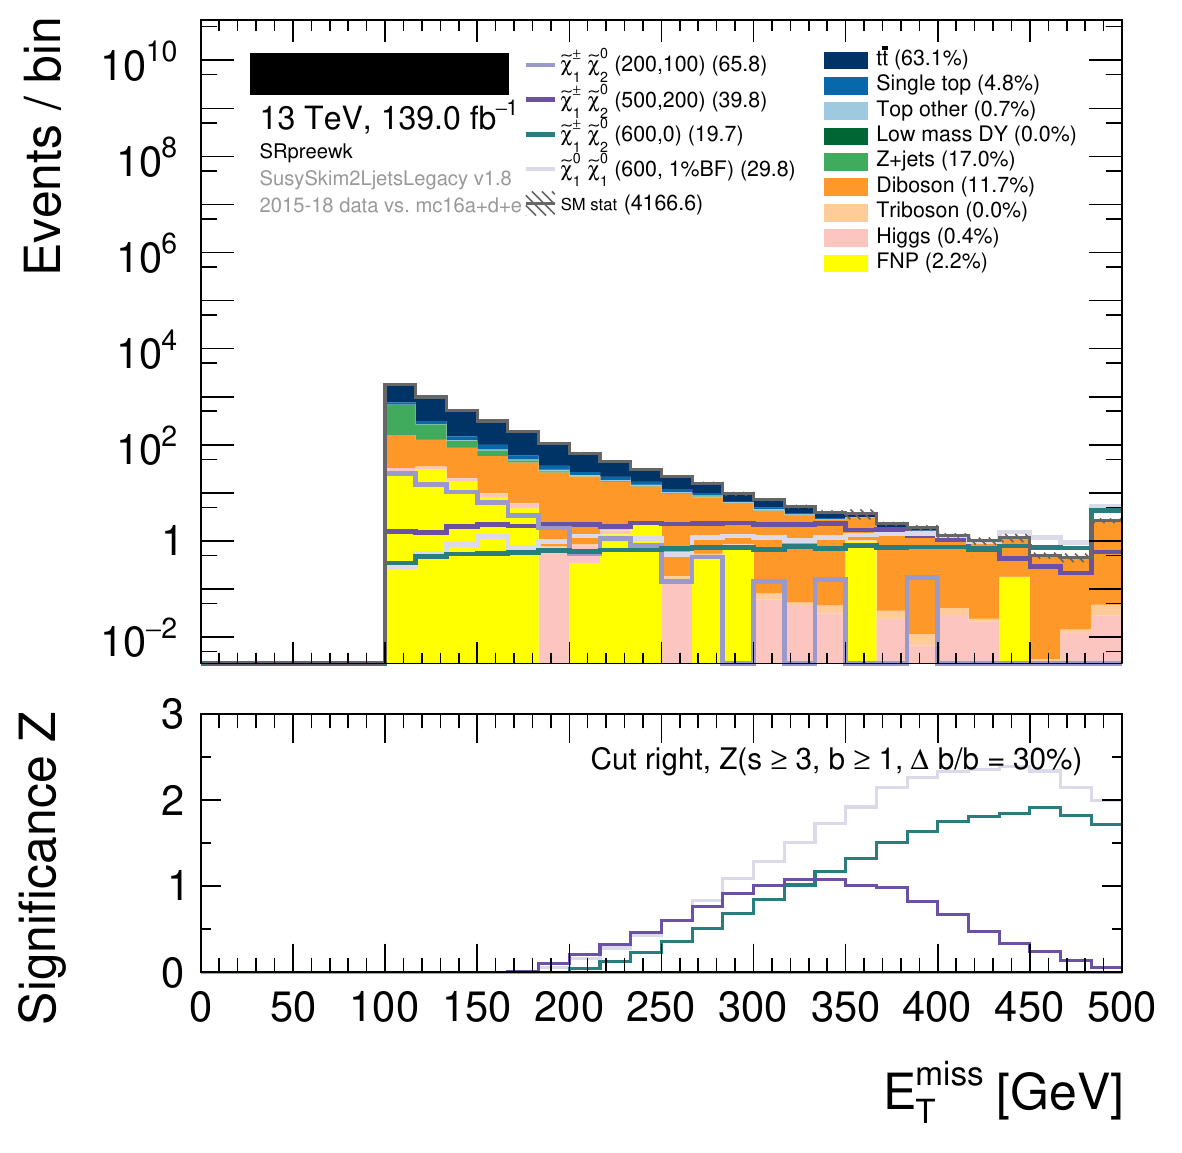
\includegraphics[width=0.49\textwidth]{figures/2ljets_presel_met_logy.png}
\hfill
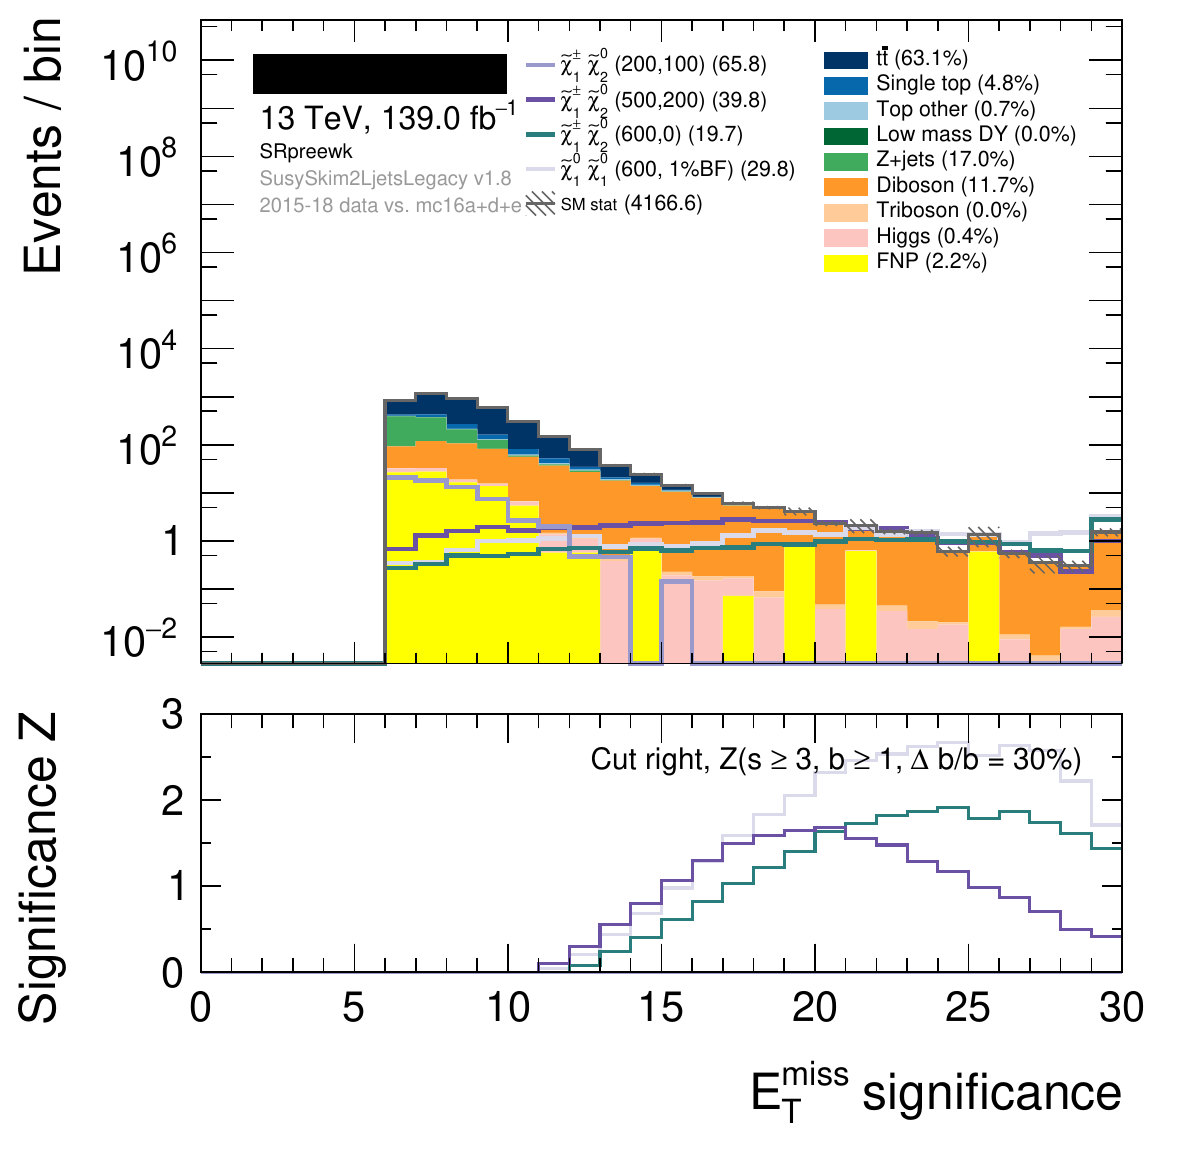
\includegraphics[width=0.49\textwidth]{figures/2ljets_presel_met_sig_logy.png}
\caption{
Illustration of how $\etmisssig$ beats $\etmiss$ alone in sensitivity to
example signal models.
At large $\etmisssig$, $t\bar t$ and other backgrounds are suppressed, leaving
quite pure diboson backgrounds and greater significance measures.
Signal models with smaller mass splittings tend to have the bulk of their
events at smaller $\etmiss$.
\\[0.5em]
This loose selection ``SRpreewk'' requires two same-flavor opposite-sign
signal leptons with
$\mll \in (71, 111)~\eV[G]$,
$\mjj \in (60, 110)~\eV[G]$,
$\nbtag \leq 1$,
$\etmiss > 100~\eV[G]$, and
$\etmisssig > 6$.
\\[0.5em]
``Significance'' displayed in the lower subplot uses the Binomial significance
$Z_{Bi}$ from~\cite{cousins2008evaluation}, with a $30\%$ background
uncertainty and yields taken to the right of a given value.
Large values indicate expected sensitivity to the signal model.
}
\label{fig:2ljets_presel_met}
\end{figure}



% CRs go in with relevant SR category
\subsection{High}

\subsection{Intermediate}

\subsection{Low}

\subsection{Off-shell}

\subsection{Discovery}

\section{Modelling}
% TODO backgorund samples
% TODO matrix method fakes
% TODO GMSB reweighting
% TODO off-shell plus/minus split
% TODO generator filtering

\subsection{Fake/non-prompt leptons}

\section{Validation}

\section{Systematics}

\section{Results}


